\chapter{Methodology}\label{chapter:methodology}

As described in the previous sections, the aim of this work is to make developers aware of the energy consumption of their programs. By using a simple and practical tool, they can quickly and accurately estimate their program's energy consumption. This allows them to get immediate feedback on energy consumption with every code change, facilitating energy-efficient development. It's important to note that this tool serves as a guide, providing energy consumption estimates to raise awareness rather than dictate action. Ultimately, it is up to developers to decide whether to prioritize performance, energy efficiency or any other factor. For example, if a program only needs to run within a certain timeframe and can afford a slight reduction in performance, developers may choose to trade some performance for improved energy efficiency, making more informed decisions thanks to the insights provided by the tool.

To provide this insight to developers it is necessary to build a tool that can provide all of that. The tool needs to be practical, which means that integrating it in an IDE is recommended. With this the developer only needs to download an extension for an IDE and will access to the insights provided by the tool.
The tool will be an extension using Language Server Protocol (LSP), so it can be integrated in all the IDEs that support this feature (VScode, Eclipse, Neovim, IntelliJ IDEA). This will make it accessible to most developers wanting feedback on the energy consumption. To make it fast, it will use static analysis to parse the code into an AST, from there it's capable of analyzing the code and using an inference function it will output the estimated cost.

Many devices rely on Java and the JVM, so it is important that the code they run is energy efficient. Several factors can affect the power consumption of Java applications, including the behavior of the garbage collector and the efficiency of the memory management system \cite{10.5555/1267847.1267870} making it difficult to predict the power consumption of Java programs. This unpredictability highlights the need for a specialized tool to accurately measure and analyze power consumption so that developers can optimize their applications for energy efficiency.
Java is an excellent choice for developing this tool because of its high interoperability with various operating systems and its widespread usage across the globe, making it a reliable and option. It has a wide range of useful libraries (JRAPL, JoularJx, Jalen) that help to measure energy accurately, and Java's typing and object-oriented features make the code easier to maintain and extend, so the tool can evolve with new energy metering standards and technologies. 

There are several Java parsing tools available, such as WALA\cite{wala_main}, SootUp\cite{sootup_main}, and Spoon\cite{spoon_main}. WALA and SootUp are primarily designed for analyzing Java Bytecode and are generally more complex to use. For this project, Spoon was chosen because it is a user-friendly tool that facilitates easy retrieval and manipulation of the AST from Java source code.

\section{Step 1: Program Generation} \label{sec:work_step1_program_generation}

In order to be able to predict energy using ML models it is of course needed a lot of data, so the models can train, and the results can be analyzed. To obtain a considerable amount of data a program generator was built.
The program generator works alongside with Java Spoon to make it the more general as possible allowing custom programs to be massed generated.
The generator works for custom Java classes or for some collections (Lists, Sets, Maps), and it can be called to analyze all the public methods of the class or just specific ones.
It starts by reading a custom Java file (or just access the Lists, Sets, Maps classes), and using Spoon it finds every public method available in the provided class. If it is needed to analyze a specific method, the generator will search in the class for every method with the name requested. Now it has access to all the public methods in the class and what parameters they receive. Since it has access to the whole custom class, it can see how its constructors are called, and use them if any of the methods parameters requires. It recursively calls constructors if needed, making it very versatile to use. After identifying the methods that will be targeted, it starts by creating templates for each of them. It creates the template to have the necessary variables needed to run the specific method, and the template is also carefully structured to function with the orchestrator that will extract the energy profile for each program, that will be explained in the next step. With the template created it is possible to create multiple programs from it. The template has some placeholders, for example to change the type or to change the size of some variable, and they will be replaced with values. By replacing the values of the template and its types, it is possible to generate multiple programs from a template that calls a specific method.

The types used by the generator are the Java wrapper classes, which are object representations of the primitive types. Using these types it is possible to achieve a more general generator, as every program can use them and if other costum types were used it would make the generator more complex and not general.

A very important aspect of the program generator is the inputs it generates. Every method works differently, and receives different parameters, and even when changing the values of these parameters, the method can behave completely different. So, this generator has an intermediate step, between the creation of the template and creating multiple programs, that finds the maximum size the input parameters should receive. Knowing the maximum size the different parameters can have is very important as it needs to be big enough, so the energy profiles can be abundant, but not to big so that the programs start to get out of memory or taking too much time to complete.
The way it works is by using binary search. It has a maximum valid input defined, and it   

\begin{comment}
\section{Step 1: Energy Profiling} \label{sec:work_step1_energy_profiling}

To give energy consumption estimates, first it is necessary to obtain energy profiles~\cite{10.1145/2884781.2884869,8816747}, so the inference function can obtain the most accurate results possible. The goal in this step is to first obtain energy profiles of collections and APIs that are widely used, break them down to their smallest functions, and understand their energy behavior. From there, it is possible to build from these granular functions to more complex and interconnected functions, ultimately covering the entire API set in detail. So whenever an API call is detected in the code, pre-built energy profiles are already available for it.
For that, a process was created in order to efficiently obtain the energy usage of code snippets.
The process uses an orchestrator that is responsible for invoking the target program and the measurement tool (PowerJoular) to accurately measure the energy consumption of the program or the specific computation being analyzed within it.

The workflow of this step can be described as follows:

\begin{itemize}
  \item The orchestrator launches a command to start the target Java Program and waits a signal.
  \item The Java program starts and setup the necessary elements to run (starting threads, reading/writing files, etc.) and then before starting the computation it wants to measure, it sends a start signal to the orchestrator to start monitoring, and waits for 100 milliseconds.
  \item The orchestrator receives the start signal and reads the PID and number of runs the target computation is going to take, which is stored in a file during the target program setup. And, finally, it starts PowerJoular using that PID. Then it waits for the stop signal.
  \item The Java program will run until it finishes the computation and then, send a stop signal back.
  \item The orchestrator on receiving the stop signal, first stops PowerJoular and then stops the target program, if needed. Then it parses the target program to extract its features, combines them with the energy information stored in the files created by PowerJoular, stores it in a CSV file and displays the energy on the screen.
\end{itemize}

The process described is responsible for generating energy profiles of various programs and storing them in a CSV file, which will be used later for training the ML model.

This allows for more precise energy measurements, avoiding reading the JVM startup, and focusing only on the computation between the signals. The workflow is more clearly illustrated in Figure \ref{fig:orchestrators_process}.

\begin{figure}
  \centering
  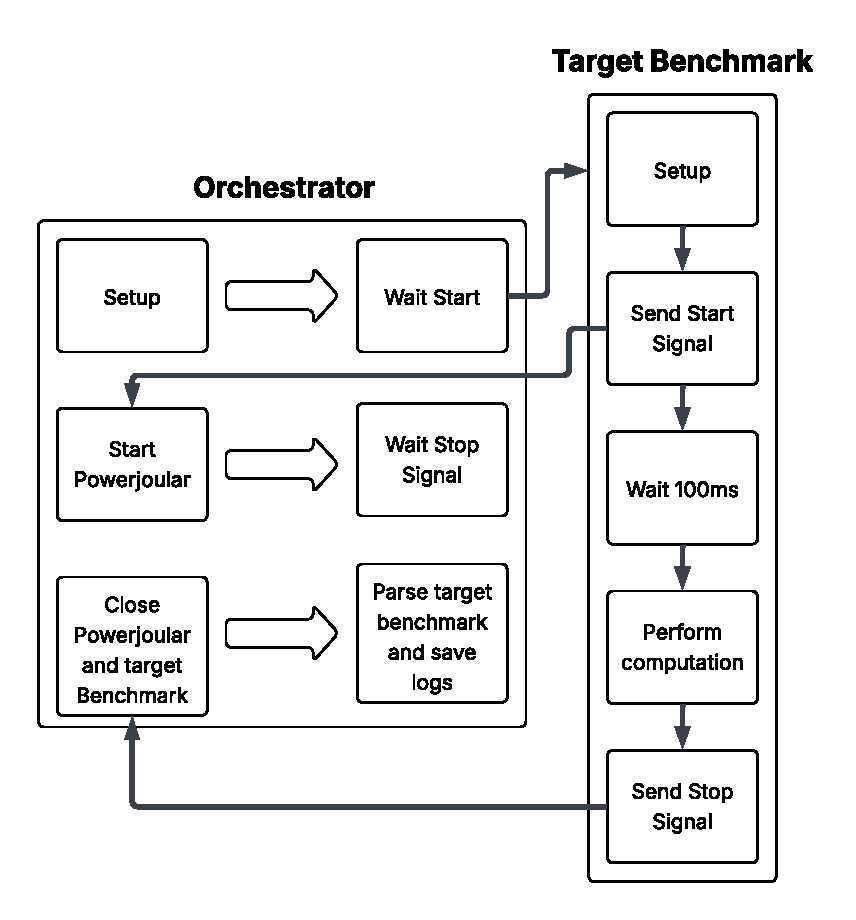
\includegraphics[width = 0.4 \textwidth]{figures/orchestrators_process.pdf}
  \caption{Orchestrator Workflow}
  \label{fig:orchestrators_process}
\end{figure}

The same workflow will be repeated across multiple machines to gather data from as many locations as possible. This approach ensures that the model developed in the next step will generate accurate outputs applicable to a wide range of machines and scenarios.


\section{Step 2: Energy Inference Function} \label{sec:work_step2_energy_inference_function}

\begin{figure}%[h]
  \centering
  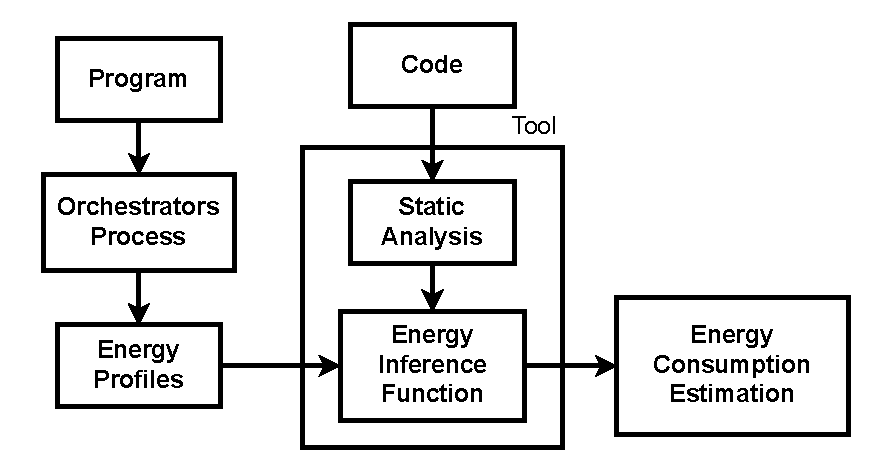
\includegraphics[width = 0.4 \textwidth]{figures/energy_inf_fun.pdf}
  \caption{Energy Inference Function}
  \label{fig:energy_inference_function}
\end{figure}

The inference function will receive as input the energy profiles obtained previously and the code that the developer wants to analyze. On receiving the code, static analyzes will be used in order to inspect the code using a Java parser (Spoon), which will provide the AST. Later this AST will be used to feed a machine learning model with the return types of the function, parameters used, loops and so on, alongside with the energy profiles. After that the model will output the estimated energy values to be displayed to the developer.
As explained in \ref{sec:background_machine_learning}, there are several ways of implementing an ML model. In this particular case, supervised ML is the best approach as it allows to train the model on previously collected energy profiles that contain the code and the energy consumed for that code. With these in mind, it is possible to test different algorithms, like the ones described in \ref{sec:background_machine_learning}, to achieve the best estimation possible.


The model will be trained using a variety of energy profiles and code inputs from different devices to achieve the most accurate energy estimates possible. This approach will improve its accuracy across devices with different hardware and software configurations.
The estimation will be the total energy used by the program, the total energy used for each function and the snippets of the function that spend the most energy.
The Figure \ref{fig:energy_inference_function} helps to visualize the function.
\end{comment}


\section{Step 3: Implementation and testing} \label{sec:work_step3_implementation_and_testing}

Once the main components of the tool are built, they need to be assembled into the extension. When using it, the developers should be able to see the total energy estimate of their code in the IDE, and it should also show the estimates for each function and its most energy consuming lines.
The estimate alone may be enough to understand if the code is high or low in energy consumption, for example, if the developer has two implementations of the same function and they both give different values, it may be easy to understand which one consumes the most. However, this may not always be the case, so the tool will also provide some information to help the developer know how good or bad the energy efficiency of the code is.

Another important step is to test and ensure that the tool performs as expected on most machines, delivers the most accurate estimations possible, and undergoes a final comparison with other tools to evaluate its effectiveness.
